\problemname{The Board Game}
Ann-Charlotte and Berit have invented their own board game.
The game is played with a board of size $N \times M$ and a chainsaw, and is intended for two players.
They players take turns making a move until one of them cannot make a move, that player loses.
A move works the following way:

The player who's turn it is chooses a horizontal or vertical line, and splits the board along it into two non-empty parts.
This can only be done at integer coordinates (so that the two resulting board pieces have integer dimensions).
The other player then chooses which of the pieces the game should continue on, while the other board piece is thrown away.
Since the dimensions always have to be integers, the loser will always be the one who's turn it is to use the chainsaw when the board has size $1 \times 1$.

Given the size of the original board, and the fact that Ann-Charlotte always starts, can you determine who wins if both players play optimally?

\begin{figure}[ht!]
\centering
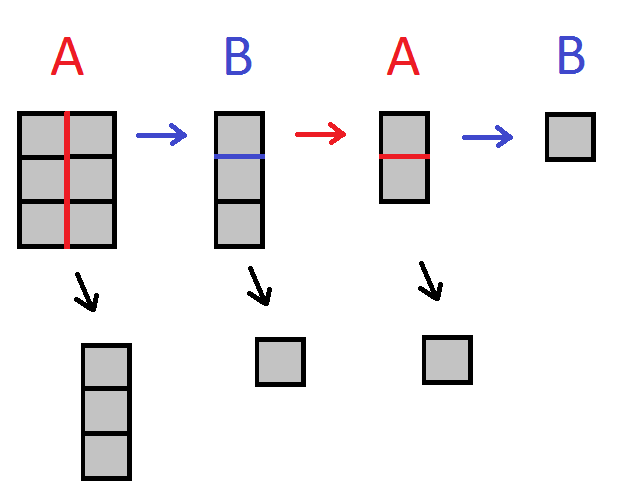
\includegraphics[width=0.6\textwidth]{bradspelet.png}
\caption{An illustration of the first example}
\label{overflow}
\end{figure}

\section*{Input}
Input consists of one line containing the two numbers $N$ and $M$ ($1 \le N,M \le 100$).

\section*{Output}
One line with the letter ``\texttt{A}'' if Ann-Charlotte wins and ``\texttt{B}'' if
Berit wins, given that they both play optimally. More precisely, if Ann-Charlotte
can win no matter how Berit plays you should write ``\texttt{A}'', otherwise you
should write ``\texttt{B}''.

\section*{Scoring}
Your solution will be tested on several groups of test cases. To get points for a group you need to pass all the tests of that group.

\noindent
\begin{tabular}{| l | l | l |}
	\hline
	Group & Points & Constraints\\ \hline
 $1$    & $20$        & $N, M \le 10$ \\ \hline
 $2$    & $80$        & No additional constraints \\ \hline
\end{tabular}

\section*{Explanation of sample 1}
In the first example $A$ wins by splitting the board into two pieces of size $1 \times 3$.
No matter what $B$ does afterwards, $A$ will get to choose between pieces of size $1 \times 2$
and $1 \times 1$. The correct strategy is to pick $1 \times 2$ (the other option immediately leads
to defeat). $B$ will then be forced to choose between two pieces of size $1 \times 1$, which both
will result in defeat for $B$.
